\documentclass[12pt]{article}

\usepackage[utf8]{inputenc}
\usepackage{datetime}
\usepackage{amsthm}
\usepackage{amsmath}
\usepackage{amssymb}
\usepackage{enumitem}
\usepackage[USenglish]{babel}
\usepackage{matlab-prettifier}
\usepackage{graphicx}
\usepackage[makeroom]{cancel}
\usepackage{bbm}

\newcommand\independent{\protect\mathpalette{\protect\independenT}{\perp}}
\def\independenT#1#2{\mathrel{\rlap{$#1#2$}\mkern2mu{#1#2}}}

\newtheoremstyle{colon}{\topsep}{\topsep}{}{}{\bfseries}{:}{ }{}
\theoremstyle{colon}
\newtheorem{exercise}{Exercise}
\newtheorem*{answer}{Answer}

\title{ORFE 523: Conic and Convex Optimization \\ Homework 3}
\author{Zachary Hervieux-Moore}

\newdate{date}{30}{03}{2017}
\date{\displaydate{date}}

\begin{document}

\maketitle

\clearpage

\begin{exercise}
  \leavevmode
  \begin{enumerate}[label=\arabic*)]
    \item Solve the following problem
      \begin{gather*}
        \min_{a, b, \eta} \lVert a \rVert + \gamma \lVert \eta \rVert_1 \\
        \text{s.t. } y_i (a^T x_i - b) \geq 1 - \eta_i \ \forall i = 1, \mathellipsis, m \\
        \eta_i \geq 0 \forall i = 1, \mathellipsis, m
      \end{gather*}
      For $\gamma = 0.1, 1, 10$, What is the optimal $a^*$ and $b^*$ for each $\gamma$?

    \item Which $\gamma$ gives the best success rate in terms of prediction? Take a look at the entries of $a^*$ in this case, what does this suggest about the people who vote for Hillary compared to those who vote for Bernie?
  \end{enumerate}
\end{exercise}

\begin{answer}
  \leavevmode
  \begin{enumerate}[label=\arabic*)]
    \item The code used to generate the optimal values is below. Table 1 shoes the optimal values for each $\gamma$.
      \begin{center}
        \begin{tabular}{|c|c|c|}
          \hline
          $ \gamma $ & $a^*$ & $b^*$ \\
          \hline
          0.1 & (0.141, 0.183, -0.723, -0.110, 0.381) & -3.147 \\
          \hline
          1 & (0.209, -0.979, -1.620, -0.460, 3.769) & -9.241 \\
          \hline
          10 & (0.151, -0.913, -1.524, -0.464, 4.821) & -8.805 \\
          \hline
        \end{tabular}
      \end{center}

    \item Table 2 shows the success rate for each $\gamma$. When $\gamma = 0.1$, this gives the best success for prediction. Using part 1), this suggest that people who have higher incomes, Hispanics, and those who live in high density areas (cities) vote for Hillary. Conversely, white demographics and those who pocess a Bachelor's degree tended to vote for Bernie.

      \begin{center}
        \begin{tabular}{|c|c|}
          \hline
          $ \gamma $ & Rate \\
          \hline
          0.1 & 0.952 \\
          \hline
          1 & 0.9048 \\
          \hline
          10 & 0.9048 \\
          \hline
        \end{tabular}
      \end{center}

      \textbf{Code Appendix}

      \begin{lstlisting}[style=Matlab-editor, basicstyle=\scriptsize]
        clear;
        clc;
        X = load('Hillary_vs_Bernie.mat');

        cvx_begin
            variable a(5);
            variable b(1);
            variable eta(175);
            % Vary this
            gamma = 0.1;

            minimize(norm(a) + gamma*norm(eta, 1));

            subject to

            for i = 1:length(X.features_train)
              X.labels_train(i)*(a'*X.features_train(i,:)' - b) >= (1 - eta(i));
                eta(i) >= 0;
            end
        cvx_end

        correct = 0;

        for i = 1:length(X.features_test)
            if(sign(a'*X.features_test(i,:)' - b) == X.labels_test(i));
                correct = correct + 1;
            end
        end

        correct/length(X.features_test)
      \end{lstlisting}
  \end{enumerate}
\end{answer}

\clearpage

\begin{exercise}
  The goal is to optimize radiation treatment. We have that $b_j$ is the power of beam $j$ for $j = 1, \mathellipsis, n$. We must have $0 \leq b_j \leq B^{max}$. $B^{max}$ is the maximum possible beam level. The exposure area is divided into $m$ vocels labeled $i = 1,\mathellipsis, m$. Dose $d_i$ delivered to voxel $i$ must be linear, i.e., $d_i = \sum_{j=1}^n A_{ij} b_j$. Where $A \in \mathbb{R}_+^{m \times n}$ is a known matirx. Furthermore, $D^{target}$ must be administered to each voxel, i.e., $d_i \geq D^{target}$ for $i \in \mathcal{T}$ where $\mathcal{T}$ is the target regions. Lastly, $d_i \leq D^{other}$ for non-target voxels. Generally, this isn't possible to we settle to minimize
  \begin{gather*}
    E = \sum_{i \notin \mathcal{T}} (d_i - D^{other})_+
  \end{gather*}
  \begin{enumerate}[label=\arabic*)]
    \item Show that the treatment planning problem is a linear program. Th optimization variable is $b \in \mathbb{R}^n$; the problem data are $B^{max}, A, \mathcal{T}, D^{target},$ and $D^{other}$.

    \item Solve the problem for the data in \texttt{treatment\_planning\_data.m}. Make a brief comment on what you see. $\textit{Remark:}$ The beam pattern matrix in this problem instance is randomly generated, but similar results would be obtained with realistic data.
  \end{enumerate}
\end{exercise}

\begin{answer}
  \leavevmode
  \begin{enumerate}[label=\arabic*)]
    \item The optimization problem is
      \begin{gather*}
        \min \sum_{i \notin \mathcal{T}} (d_i - D^{other})_+ \\
        \text{s.t. } d_i \geq D^{target} \ \forall i \in \mathcal{T} \\
        0 \leq b_i \leq B^{max} \\
        d_i = \sum_{j = 1}^n A_{ij} b_j
      \end{gather*}
      We have that $d_i$ is an linear function of $b$. Furthermore, $\min (x)_+$ can be turned into the following,
      \begin{gather*}
        \min \alpha \\
        \text{s.t. } \alpha \geq 0 \\
        \alpha \geq x
      \end{gather*}
      So, the objective $(\cdot)_+$ can be linearized. Thus, the above problem has a linear objective and linear constraints. The problem is the linear program below
      \begin{gather*}
        \min \sum_{i \notin \mathcal{T}} \alpha_i \\
        \text{s.t. } \sum_{j = 1}^n A_{ij} b_j \geq D^{target} \ \forall i \in \mathcal{T} \\
        0 \leq b_i \leq B^{max} \\
        0 \leq \alpha_i \\
        \sum_{j = 1}^n A_{ij} b_j - D^{other} \leq \alpha_i
      \end{gather*}
      But $\alpha_i = (\sum_{j = 1}^n A_{ij} b_j - D^{other})_+$ and so the only decision variable is really $b_i$.

    \item Figure 1 shows the histogram for voxels being targeted. Figure 2 shows the histogram for those not being targeted. The code used to generate the histograms are below. Notice that most of the voxels being targeted are above the required dose by just a little (1 to 1.2). Also, the vast majority of voxels not being targeted are under $D^{other} = 0.25$. This is exactly what we would want with a real patient.

      \begin{figure}[ht]
        \caption{Histogram for $D^{target}$}
        \centering
          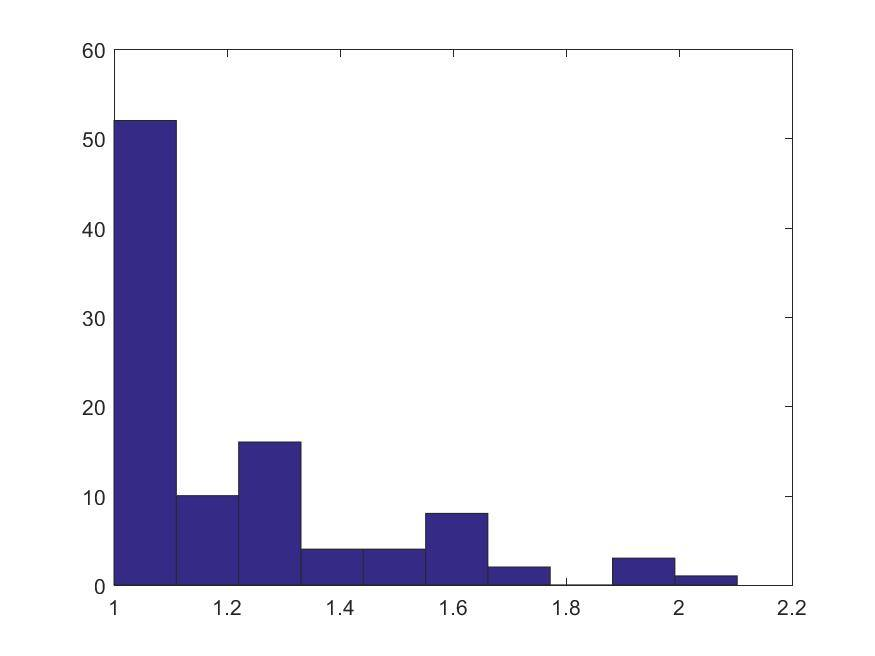
\includegraphics[width=0.8\textwidth]{dose_tumor.jpg}
      \end{figure}

      \begin{figure}[ht]
        \caption{Histogram for $D^{other}$}
        \centering
          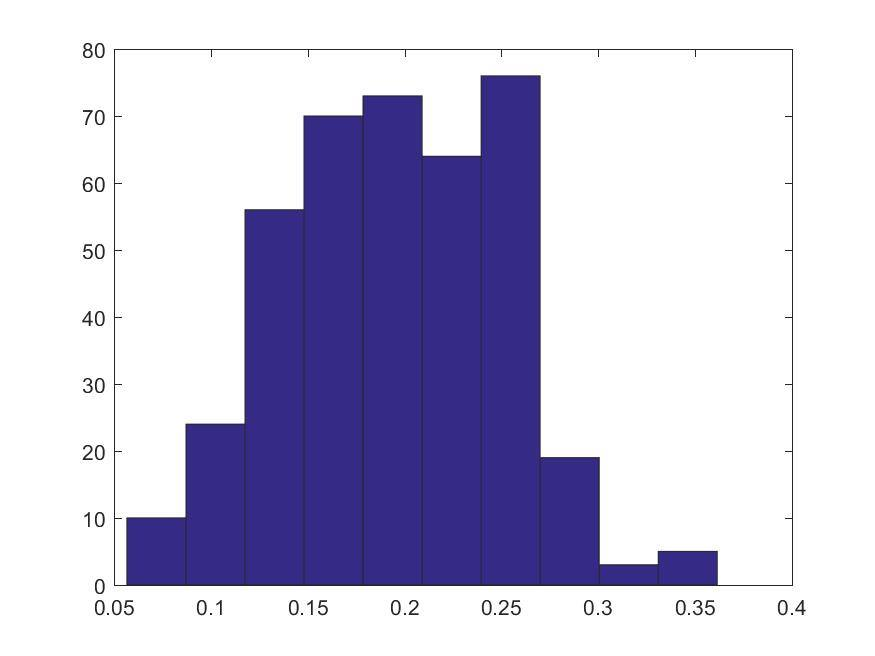
\includegraphics[width=0.8\textwidth]{dose_other.jpg}
      \end{figure}

      \clearpage

      \textbf{Code Appendix}

      \begin{lstlisting}[style=Matlab-editor, basicstyle=\scriptsize]
        clear;
        clc;
        run('treatment_planning_data.m');

        cvx_begin
            variable b(n);
            d_tumor = Atumor*b;
            d_other = Aother*b;
            minimize(sum(max(0,d_other-Dother)));

            subject to
            d_tumor >= Dtarget;
            0 <= b;
            b <= Bmax
        cvx_end

        figure1 = figure
        hist(d_tumor)
        saveas(figure1,'dose_tumor.jpg')

        figure2 = figure
        hist(d_other)
        saveas(figure2,'dose_other.jpg')

      \end{lstlisting}
  \end{enumerate}
\end{answer}

\clearpage

\begin{exercise}
  Suppose $\mathcal{G} = \{Q_1, \mathellipsis, Q_k \} \subseteq \mathbb{R}^{n \times n}$ is a group, i.e., closed under products and inverse. We say that the funciton $f : \mathbb{R}^n \rightarrow \mathbb{R}$ is $\mathcal{G}$-invariant, or \textit{symmetrix with respect to } $\mathcal{G}$, if $f(Q_i x) = f(x)$ holds for all $x$ and $i = 1, \mathellipsis, k$. We define $\bar{x} = (1/k) \sum_{i=1}^k Q_i x$, which is the average of $x$ over its $\mathcal{G}$-orbit. We define the \textit{fixed subspace} of $\mathcal{G}$ as
  \begin{gather*}
    \mathcal{F} = \{ x : Q_i x = x, i = 1, \mathellipsis, k \}
  \end{gather*}
  \begin{enumerate}[label=\alph*)]
      \item Show that for any $x \in \mathbb{R}^n$ we have $\bar{x} \in \mathcal{F}$.
      \item Show that if $f : \mathbb{R}^n \rightarrow \mathbb{R}$ is convex and $\mathcal{G}$-invariant, then $f(\bar{x}) \leq f(x)$.
      \item We say the optimization problem
        \begin{gather*}
          \min f_0(x) \\
          \text{s.t. } f_i(x) \leq 0, i = 1, \mathellipsis, m
        \end{gather*}
        is $\mathcal{G}$-invariant if the objective $f_0$ is $\mathcal{G}$-invariant and the feasible set is $\mathcal{G}$-invariant, which means
        \begin{gather*}
          f_1(x) \leq 0, \mathellipsis, f_m(x) \leq 0 \rightarrow f_1(Q_i x) \leq 0, \mathellipsis, f_m(Q_i x) \leq 0
        \end{gather*}
        for $i = 1, \mathellipsis, k$. Show that if the problem is convex and $\mathcal{G}$pinvariant, and there exists an optimal point, then there exists an optimal point in $\mathcal{F}$. In other words, we can adjoin the equality constraints $x \in \mathcal{F}$ to the problem, without loss of generality.
      \item As an example, suppose that $f$ is convex and symmetric, i.e., $f(Px) = f(x)$ for every permutation $P$. Show that if $f$ has a minimizer, then it has a minimizer of the form $\alpha 1$. (This means to minimize $f$ over $x \in \mathbb{R}^n$, we can just as well minimize $f(t 1)$ over $t \in \mathbb{R}$).
  \end{enumerate}
\end{exercise}

\begin{answer}
  \leavevmode
  \begin{enumerate}[label=\alph*)]
    \item We have that
      \begin{gather*}
        \bar{x} = (1/k) \sum_{i=1}^k Q_i x
      \end{gather*}
      Thus,
      \begin{gather*}
        Q_j(\bar{x}) = (1/k) \sum_{i=1}^k Q_j Q_i x \\
        Q_j(\bar{x}) = (1/k) \sum_{i=1}^k Q_i x = x
      \end{gather*}
      Where the second line results since $\mathcal{G}$ is a group and so closure under products implies that multiplying by $Q_j$ simply permutes the original values $Q_i$.

    \item Suppose that $f$ is convex and $\mathcal{G}$-invariant. Thus, by convexity
      \begin{gather*}
        f(\bar{x}) = f((1/k) \sum_{i=1}^k Q_i x) \leq (1/k) \sum_{i=1}^k f(Q_i x)
      \end{gather*}
      By $\mathcal{G}$-invariance
      \begin{gather*}
        = (1/k) \sum_{i=1}^k f(x) = f(x)
      \end{gather*}
      So we conclude that $f(\bar{x}) \leq f(x)$.

    \item Suppose that $x^*$ satisfies the optimization problem. By part b), we have that $f_0(\bar{x^*}) \leq f_0(x^*)$ since $f_0$ is $\mathcal{G}$-invariant. From part a), we know $\bar{x} \in \mathcal{F}$. Thus, we only have to show that $\bar{x}$ is feasible. Since the problem is convex, then $f_i(\cdot)$ is convex and so
      \begin{gather*}
        f_i(\bar{x}) \leq (1/k) \sum_{i=1}^k f(Q_i x) \\
        \leq (1/k) \sum_{i=1}^k 0 = 0
      \end{gather*}
      Where the second line if the result of $\mathcal{G}$-invariance of the feasible set. Thus $\bar{x}$ is feasible and we conclude that we can add the constraint $x \in \mathcal{F}$ with no loss in generality.

    \item If $f(P x) = x$ for every permutation $P$. Then we have that
      \begin{gather*}
        \mathcal{F} = \{ t \mathbbm{1} : t\in \mathbb{R} \}
      \end{gather*}
      Which is due to the fact that if we permute any elements of $x$ and get back $x$, then $x$ must have the same element in all of its entries. Thus, by part c), $f$ if convex and $P$-invariant, if we minimize $f$ over $x \in \mathbb{R}^n$, then we can just minimize over $x \in \mathcal{F}$. That is, we can minimize over ($t \mathbbm{1}$) such that $t \in \mathbb{R}$.
  \end{enumerate}
\end{answer}

\clearpage

\begin{exercise}
  Define $M_C$ as the following function of a convex set $C$ in $\mathbb{R}^n$:
  \begin{gather*}
    M_C(x) = \inf \{ t > 0 : \frac{x}{t} \in C \}
  \end{gather*}
  over the domain
  \begin{gather*}
    dom(M_C) = \{ x \in \mathbb{R}^n : \frac{x}{t} \in C \text{ for some } t > 0 \}
  \end{gather*}
  \begin{enumerate}[label=\arabic*)]
    \item Show that $M_C$ is a convex function.
    \item Suppose $C$ is also compact, origin symmetric ($x \in C$ if and only if $-x \in C$), and has nonempty interior. Show that $M_C$ is a norm over $\mathbb{R}^n$. What is its unit ball?
    \item Show that an even degree homogeneous polynomial is convex if and only if it is quasiconvex. (Hint: use what you proved in the previous parts of this question).
  \end{enumerate}
\end{exercise}

\begin{answer}
  \leavevmode
  \begin{enumerate}[label=\arabic*)]
    \item We have for $\lambda \in (0,1)$ and $x, y \in \mathbb{R}^n$
      \begin{gather*}
        t^* = M_C(\lambda x + (1-\lambda) y) = \inf \{ t > 0 : \frac{\lambda x + (1-\lambda) y}{t} \in C \}
      \end{gather*}
      If we show that $t^* \leq \lambda M_C(x) + (1-\lambda)M_C(y)$, then we are done. So we check that $t = \lambda M_C(x) + (1-\lambda)M_C(y)$ is feasible. Since $\lambda M_C(x) + (1-\lambda)M_C(y) > 0$, we only need to check that $\frac{\lambda x + (1-\lambda) y}{\lambda M_C(x) + (1-\lambda)M_C(y)} \in C$. We have
      \begin{gather*}
        \frac{\lambda x + (1-\lambda) y}{\lambda M_C(x) + (1-\lambda)M_C(y)} \\
        = \alpha \frac{x}{M_C(x)} + (1-\alpha) \frac{y}{M_C(y)} \\
        \text{where } \alpha = \frac{1}{1 + \frac{M_C(y)}{M_C(x)} \frac{1-\lambda}{\lambda}}
      \end{gather*}
      Clearly, $\alpha \in (0,1)$. WLOG, assume $C$ is closed so that $\frac{x}{M_C(x)}, \frac{y}{M_C(y)} \in C$, otherwise, just work with the closure of $C$. Since $C$ is convex, we then have that $\alpha \frac{x}{M_C(x)} + (1-\alpha) \frac{y}{M_C(y)} \in C$. Thus,
      \begin{gather*}
        t^* \leq \lambda M_C(x) + (1-\lambda)M_C(y) \\
        \implies M_C(\lambda x + (1-\lambda) y) \leq \lambda M_C(x) + (1-\lambda)M_C(y)
      \end{gather*}
      So $M_C(\cdot)$ is convex.

    \item We show the three properties of a norm
      \begin{itemize}
        \item (positivity) Cleary, $M_C(x) \geq 0$ since $t > 0$. Suppose we have that $M_C(x) = 0$. Since $C$ is compact, then it is bounded. By contradiction, suppose $x \neq 0$, then as $t \rightarrow 0$, then $\lVert \frac{x}{t} \rVert \rightarrow \infty$. But then this means that $M_C(x) \neq 0$ as $\lVert \frac{x}{t} \rVert$ leaves $C$ since it is bounded. Therefore, we must have that $M_C(x) = 0$ implies that $x = 0$. Note that $x \in C$ since it is non-empty and since $x$ and $-x$ are in $C$, this means that $0$ must be in $C$.

        \item (homogeneity) Suppose $M_C(x) = a$. Then $M_C(\alpha x) = \inf \{ t > 0 : \frac{\alpha x}{t} \in C \}$. By origin symmetry of $C$, if $\alpha < 0$, then $M_C(\alpha x) = \inf \{ t > 0 : \frac{- \alpha x}{t} \in C \}$. So we can consider $M_C(\alpha x) = \inf \{ t > 0 : \frac{\lvert \alpha \rvert x}{t} \in C \}$. We relabel $t' = \frac{t}{\lvert \alpha \rvert}$ to get $M_C(\alpha x) = \inf \{ t' > 0 : \frac{x}{t'} \in C \}$ and so we conclude that $\frac{M_C(\alpha x)}{\lvert \alpha \rvert} = a$ which means that $M_C(\alpha x) = \lvert \alpha \rvert M_C(x)$.

        \item (triangle inequality) We have by homogeneity of $M_C$ and convexity of $M_C$ that
          \begin{gather*}
            M_C(x + y) = M_C(2(\frac{1}{2} x + \frac{1}{2} y)) = 2 M_C(\frac{1}{2} x + \frac{1}{2} y) \leq M_C(x) + M_C(y)
          \end{gather*}

        Thus, $M_C$ is a norm if it is compact and origin symmetric with non-empty interior. Now we show what the unit ball is. Recall that $0 \in C$ since it is non-empty. By definition, $\frac{x}{M_C(x)} \in C$ since $C$ is compact (that is the infimum is achieved). Suppose that $M_C(x) \leq 1$. By convexity of $C$ we have
        \begin{gather*}
          x = M_C(x) \frac{x}{M_C(x)} + (1-M_C(x)) 0
        \end{gather*}
        But this is a convex combination of elements in $C$ and so $x \in C$. That is, if $M_C(x) \leq 1$ then $x \in C$. Also, if $x \in C$, then $M_C(x) \leq 1$ since $\frac{x}{1} = x \in C$. Thus, the unit ball is precisely $C$.
      \end{itemize}

    \item Consider the polynomial $p(x)$. Convex implies quasiconvex as shown in class. To show the converse consider the sublevel set $S_1$. Since it is a homogeneous polynomial, we also have that $p(t x) = t^d p(x)$. Thus,
      \begin{gather*}
        p(x) = \inf \{ t > 0 : \frac{p(x)}{t} \leq 1 \} \\
        = \inf \{ t > 0 : p(\frac{x}{t^{1/d}}) \leq 1 \} \text{ by homogeneity} \\
        = \inf \{ t > 0 : \frac{x}{t^{1/d}} \in S_1 \} \\
        = M_{S_1}(x)^d
      \end{gather*}
      Since $M_{S_1}$ is convex as it is a norm as shown in step 2) and $x^d$ is convex since $d$ is even. Also, $M_{S_1}$ is non-negative and $x^d$ is non-decreasing on $[0,\infty)$ we conclude that $p(x)$ is convex since it is a composition of two convex functions with the preceding properties.
  \end{enumerate}
\end{answer}

\clearpage

\begin{exercise}
  A matrix $A$ is called \textit{doubly stochastic} if $A$ is nonnegative and each of its rows and columns sum up to 1. A \textit{permutation} matrix is an integral doubly stochastic matrix. Show that every doubly stochastic matrix is a convex combination of permuation matrices. (Hint: relate this to bipartite matching).
\end{exercise}

\begin{answer}
  As per the hint, we define the following bipartite graph. Make two columns of nodes from 1 to $n$, where $n$ is the dimension of the square matrix $A$. Then create an edge of weight 1 from the node $i$ in column 1 to nodes $j$ column 2 if $A_{ij}$ is non zero. Let $X$ be the incidence matrix of this graph.

  By recreating the maximum matching linear program done in class and using the fact that the incidence matrix of a bipartite graph is TUM, then there exists a matrix $P$ that achieves maximal matching where $P_{ij} = 1$ if both nodes $i$ and $j$ are connected in the solution. Since $A$ is doubly stochastic, we have that the maximal matching has precisely a value of $n$. Since $P$ is a solution to a matching problem, then each column and row has at most one 1. We conclude that $P$ is a permutation matrix since there are $n$ rows and columns and the values must sum up to $n$.

  Now, we create a new matrix $A_1 = A - \gamma P$ where $\gamma$ is chosen such that $A - \gamma P \geq 0$. Then, by construction, $A_1$ has at least 1 more zero entry than $A$. However, $\frac{A_1}{1-\gamma}$ is still doubly stochastic ($A - \gamma P$ has row and column sums of $(1-\gamma)$) and so we can repeat the process above. We finish when we reach an iteration when $\gamma = 1$.
\end{answer}

\clearpage

\begin{exercise}
  Let $A$ be an integral matrix. Show that $A$ is totally unimodular if and only if for every integral vector $b$, the polyhedon $\{ x : x \geq 0, Ax \leq b \}$ is integral. (Hint: If $A$ is not totally unimodular, use the inverse of a submatrix which does not have determinant $\{0, -1, +1\}$ to construct an integer vector $b$ that generates a non-integral vertex in the polyhedron).
\end{exercise}

\begin{answer}
  We showed in class that if $A$ is TUM, then the polyhedron $P = \{ x : x \geq 0, Ax \leq b \}$ is integral. Now, suppose that $A$ is not TUM. Then, this means that there is a submatrix $B$ of $A$ which does not have a determinant in $\{-1, 0, +1\}$. Furthermore, since $A$ is integral, the determinant of $B$ is also integral (since the determinant is an integral function of the entries). However, since $\lvert det(B) \rvert > 1$, then we must have that $det(B^{-1}) = \frac{1}{det(B)}$ is not an integer. This implies that $B^{-1}$ has a non integer entry, because if it had all integer entries, its determinant would be integral.

  Suppose that the non integer entry of $B$ is in its $j^{th}$ column. Now, let us define $x$ that satisfies
  \begin{gather*}
    B^{-1} e_j = x
  \end{gather*}
  Where $e_j$ is the canonical basis vector. Then we have that $x$ is non integral. We correct the case where $x$ has negative entries. Thus, we must add a sufficiently large integral $y$ to $x$ to make it non negative
  \begin{gather*}
    x = B^{-1} e_j + y
  \end{gather*}
  Now suppose $b = e_j$,
  \begin{gather*}
    \implies B x = b + B y
  \end{gather*}
  Note that $b + B y$ is still integral for suitably chosen $y$. However, we still must correct for the dimension difference between $B$ and $A$. Without loss in generality, assume that $B$ is the upper left $k \times k$ block of $A$. Thus, we pad our $x$ to be
  \begin{gather*}
    x^* = \begin{bmatrix} x \\ 0 \\ \vdots \\ 0 \end{bmatrix}, b^* = \begin{bmatrix} b \\ * \\ \vdots \\ *  \end{bmatrix}
  \end{gather*}
  Where the $*$'s in $b$ are chosen integers that are larger than the $n-k$ bottom rows of $Ax$. Thus, we have
  \begin{gather*}
    A x = \begin{bmatrix} b + B y \\ * \\ \vdots \\ * \end{bmatrix} \leq b^*
  \end{gather*}
  This $x$ is indeed a vertex. This is because we have $k$ binding constraints from $Ax \leq b$ since our construction leads the first $k$ rows of $Ax$ to be equal $b$. We also have $n-k$ binding constraints from the $n-k$ entries of $x$ which are 0. Thus, this $x$ is specified by $n$ constraints and hence this is a vertex. We conclude that $b$ is not integral and thus if $A$ is not TUM then there exists a $b$ such that the polyhedron is not integral.
\end{answer}

\end{document}